\documentclass[3pt,twocolumn]{elsarticle}
\usepackage[spanish]{babel}
\usepackage[utf8]{inputenc}
\usepackage[T1]{fontenc}
\usepackage{lineno,hyperref}
\modulolinenumbers[5]
\usepackage{graphicx}
\usepackage{subcaption}
\usepackage{listings}
\lstset{language=R, breaklines=true}
\usepackage{amsmath}
\bibliographystyle{elsarticle-num}
\captionsetup[subfigure]{labelformat=brace}

\makeatletter

\renewenvironment{abstract}{\global\setbox\absbox=\vbox\bgroup
  \hsize=\textwidth\def\baselinestretch{1}%
  \noindent\unskip\textbf{Resumen}  % <--- Edit as necessary
 \par\medskip\noindent\unskip\ignorespaces}
 {\egroup}

\def\keyword{%
  \def\sep{\unskip, }%
 \def\MSC{\@ifnextchar[{\@MSC}{\@MSC[2000]}}
  \def\@MSC[##1]{\par\leavevmode\hbox {\it ##1~MSC:\space}}%
  \def\PACS{\par\leavevmode\hbox {\it PACS:\space}}%
  \def\JEL{\par\leavevmode\hbox {\it JEL:\space}}%
  \global\setbox\keybox=\vbox\bgroup\hsize=\textwidth
  \normalsize\normalfont\def\baselinestretch{1}
  \parskip\z@
  \noindent\textit{Palabras clave: }  % <--- Edit as necessary
  \raggedright                         % Keywords are not justified.
  \ignorespaces}

\def\ps@pprintTitle{%
     \let\@oddhead\@empty
     \let\@evenhead\@empty
     \def\@oddfoot{\footnotesize\itshape
       Facultad de Ingeniería Mecánica y Eléctrica \ifx\@journal\@empty % <--- Edit as necessary
       \else\@journal\fi\hfill\today}%
     \let\@evenfoot\@oddfoot}

\makeatother

\begin{document}

\twocolumn[
\begin{@twocolumnfalse}
\begin{frontmatter}
\title{Simulación de empaquetamiento de objetos utilizando algoritmo genético}
\author{Susana Ruiz Nuñez}
\address{susanaruiznnz@uanl.edu.mx}
\address{Maestría de Ingeniería en Sistemas, Universidad Autónoma de Nuevo León}

\begin{abstract}
Los problemas de empaquetamiento de objetos y la asignación de objetos a una mochila tienen gran aplicación en la industria actual, sobre todo en la de fabricación, logística y nanotecnología. La optimización del empaquetado puede llevar a minimizar los costos que provoca el uso desmedido de materias primas, lo que da valor adicional al producto final. Con el aumento del uso de las tecnologías se hace cada vez más presente la importancia del desarrollo en las áreas de investigación operativa e ingeniería de la producción. Existen un número reducido de publicaciones acerca del tema de empaquetamiento y menos aún publicaciones donde aborden el uso de algoritmos genéticos. Este proyecto tiene como objetivo principal realizar una comparación entre modelos heurísticos y un algoritmo genético para la resolución de problemas de mochila y empaquetamiento. Para ello se propone un modelo basado en algoritmo genético para un empaquetamiento más eficaz. Se obtiene de la comparación que el modelo propuesto es más rápido a la hora de hallar una solución pero que muy pocas veces llega a la mejor solución.
\end{abstract}

\begin{keyword}
Empaquetamiento \sep mochila \sep simulación \sep algoritmo genético
\end{keyword}
\end{frontmatter}
\end{@twocolumnfalse}
]

\section{Introducción}
Es bien sabido que incluso la versión unidimensional del problema de encontrar el óptimo al uso de un recurso dado, el problema clásico de la mochila, pertenece a la clase de NP-difícil de Problemas de optimización. Por esta razón, la mayor parte del trabajo relacionado con problemas de corte y embalaje emplean enfoques heurísticos \cite{aline}. 

Se conoce un método denominado algoritmo genético que consiste en métodos adaptativos generalmente usados
en problemas de búsqueda y optimización de parámetros, basados en la reproducción sexual y en el principio de supervivencia del más apto \cite{marcos}.
Para este trabajo se quiere hacer una unión entre ambos términos para lograr
un modelo con mayor eficiencia a la hora de resolver los problemas de empaquetamientos.

\section{Antecedentes}
El problema de empaquetamiento en un rectángulo con dimensiones abiertas es conocido como Bin Packing Problem. En este problema un conjunto de objetos (por ejemplo, polígonos convexos o círculos) se debe cortar de una faja o placa de forma rectangular. Los objetos pueden ser orientados libremente. Existen dos formas a mencionar; cuando las placas de diseño necesitan ser producidas, o se encuentran ya disponibles en stock \cite{andreas}. El objetivo es minimizar el área de los rectángulos de diseño. Las placas de diseño están sujetos a los límites inferior y superior de sus anchos y longitudes
\cite{luiz}.
\begin{figure}[ptb]
	\begin{center}
		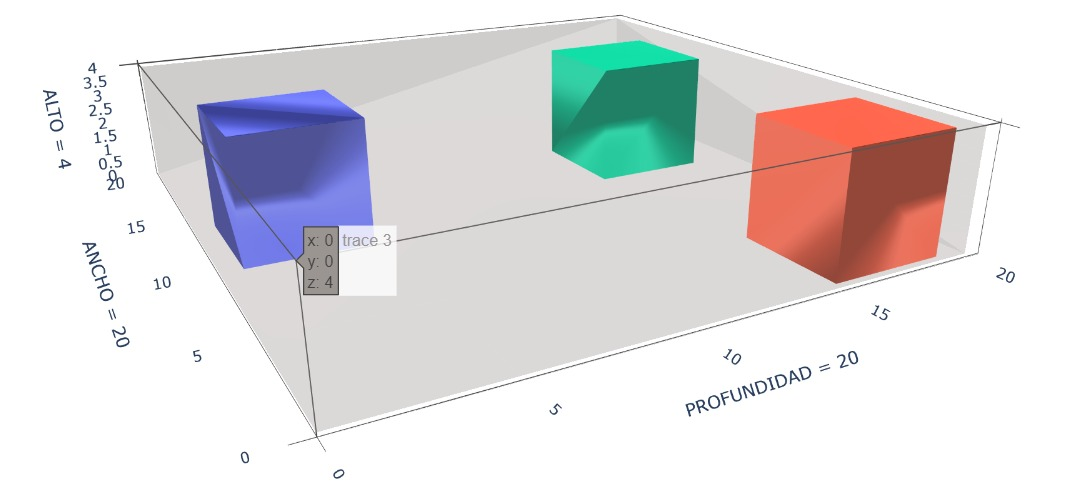
\includegraphics[width=\linewidth]{Imag1.jpeg}
	\end{center}
	\caption{Empaquetamiento utilizando librería plotly de Python.\label{rmsf}}
\end{figure}
Se utilizan la mayoría de los enfoques que se ocupan de la interacción de dos (o algunos) objetos en algoritmos de colocación para instancias más grandes como reglas de decisión local \cite{benel}. Algunos de los primeros enfoques a problemas de empaque irregular utilizaron la estrategia de agrupar las primeras piezas dentro de formas más fáciles de manejar \cite{litv}.  
\section{Trabajos relacionados}
Se encontró mientras se desarrollaba la investigación para este proyecto algunos trabajos relacionados que tuvieron acto impacto en la elaboración del mismo. Tal es el caso de (Enríquez, 2017) que presenta para un caso de industria una solución mediante algoritmo genético para el problema de asignación de la mochila \cite{gladys}.
Otro trabajo que se utilizó como fuente fue el de (Soto, 2011) que plantea un algoritmo de optimización para el problema de la mochila multidimensional \cite{soto}.  
\section{Modelo propuesto}
El modelo que se propone parte de las características generales de un problema de mochila. Donde matemáticamente se expresan las restricciones y se definen las variables. Se parte de que el problema puede ser formulado como un vector de variables binarias $X_i$.
\begin{equation}
	X_i = \text{1 Si el elemento i es seleccionado, 0 otro caso}  
\end{equation} 
Otros elementos a tener en cuenta como parte de las restricciones fueron los pesos y por consiguiente la cantidad de objetos que se podían empaquetar. En el modelo matemático general se tiene que $p_i$ sería la ganancia de un elemento, $w_i$ el tamaño de dicho elemento y aquí se nombra a $v$ el tamaño de la mochila,
\begin{equation}
	\sum_{i=1}^{n} w_i x_i \leq v,
\end{equation}
\begin{equation}
	 x_i \in \{0,1\}, i = 1, ..., n ,
\end{equation}
y por supuesto teniendo en cuenta finalmente la función objetivo.
\begin{equation}
	\sum_{i=1}^{n} p_i x_i.
\end{equation}
Tomando en cuenta la base del algoritmo genético \cite{satu} el problema se entiende de la siguiente manera,  se cada individuo representa un vector de asignación de elementos en la mochila xj y la factibilidad del mismo se evalúa en base al valor de la función objetivo, con los respectivos valores de las variables xj. Si la asignación cumple con las restricciones de capacidad la solución recibe el valor de la función objetivo correspondiente. 
Este algoritmo se ejecutó primeramente para 100 iteraciones, para luego quedarse en 50 iteraciones.
\subsection{Implementación y experimentación}
La simulación se realizó en una laptop HP con un procesador AMD Ryzen 3 con 4 GB de memoria Ram y con un sistema operativo de 64 bits. Para la aplicación del modelo propuesto se trabajó con el lenguaje Python en su versión 3.8. \\ 
Para este trabajo se utilizaron instancias de las librerías citadas \cite{beasley} de casos reales de diferentes problemas de mochila unidimensional y de varias dimensiones. 
 

\section{Resultados}
Se muestra como resultado en la Figura 2 que el algoritmo genético no llegó a alcanzar el mejor valor para resolver la situación dada. En un primer instante se hizo el análisis para un número mucho mayor de iteraciones o generaciones, pero como se observa en la figura, a partir de las primeras iteraciones (de las número seis para ser mas precisos) el algoritmo converge y casi encuentra su mejor valor, por lo que se obtuvieron dos conclusiones importantes; la primera, que era necesario reducir el número de iteraciones y segundo que el algoritmo es notablemente rápido a la hora de encontrar una solución.
\begin{figure}[ptb]
	\begin{center}
		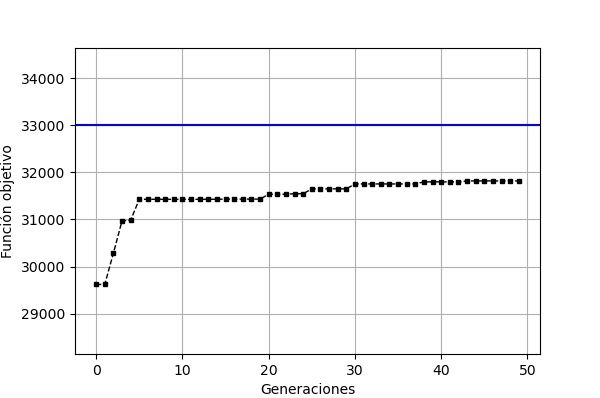
\includegraphics[width=\linewidth]{Figure_1.png}
	\end{center}
	\caption{Desempeño del algoritmo genético.\label{rmsf}}
\end{figure}

A continuación se muestran datos que se pidieron que diera el programa que refuerzan los resultados mostrados hasta ahora. Se nota la rapidez del algoritmo en llegar a la mejor solución posible que él puede entregar pero sigue viéndose que no alcanza los valores deseados.
\begin{table}[h]
	\begin{center}
		\caption{Datos del valor óptimo y el tiempo de ejecución de ambos algoritmos.}
		\label{pdb}
		\begin{tabular}{r r}
			\hline
			Algoritmo & Valor óptimo 32995.069\\
			& Tiempo de ejecución 1.530 seg\\
			\hline
			Algoritmo genético & Valor óptimo 31818.455 \\
			& Tiempo de ejecución 0.577 seg\\
			\hline
		\end{tabular}
	\end{center}
\end{table}

\section{Trabajo futuro}
Este proyecto fue realizado con el acercamiento al área de simulación utilizando algoritmos genéticos teniendo en cuenta algunas restricciones en el modelo propuesto. Queda como proyecto futuro seguir abordando en el tema incluyendo más restricciones que puedan aparecer en un problema de este tipo. La mayor parte del trabajo relacionado con problemas de empaquetamiento que se ha visto hasta ahora emplean enfoques heurísticos por lo que queda trabajo pendiente en el desarrollo de métodos de solución exactos para ampliar la gama de casos óptimos solucionables.

\section{Conclusiones}
Se concluye así que el algoritmo genético se debe utilizar para resolver problemas de empaquetamiento  cuando se requiere unos datos iniciales lo más cercanos al valor deseado de forma rápida pero no para perseguir el mejor valor que de solución al problema.

\section{Agradecimientos}
Se da un agradecimiento a la Dra. Elisa quien contribuyó directamente en el diseño del modelo de este trabajo, el cual fue realizado como culminación del curso de Simulación de la Facultad de Ingeniería Eléctrica y Mecánica de la Universidad Autonóma de Nuevo León.

\bibliography{Bibliografia}

\end{document}